\documentclass{article}

\usepackage[english]{babel}
\usepackage{float}
\usepackage[letterpaper,top=2cm,bottom=2cm,left=3cm,right=3cm,marginparwidth=2cm]{geometry}
\usepackage{amsmath}
\usepackage{amssymb}
\usepackage{graphicx}
\usepackage{grffile}
\usepackage{booktabs}
\usepackage{array}
\usepackage{tabularx}
\usepackage{caption}
\usepackage{verbatim}
\usepackage{xcolor}
\usepackage{fancyvrb}
\captionsetup[figure]{justification=centering}
\usepackage[colorlinks=true, allcolors=blue]{hyperref}
\setlength{\emergencystretch}{3em}

\title{\textbf{ME 144L Lab 9: PMDC Motor Modeling, Drives, and Sensing}}
\author{Alejandro Diaz \\ TA: Gabrielle Naquila}
\date{April 13, 2026}

\begin{document}
\maketitle

% =======================================================
\section{Back-EMF Regression and Motor Constant}
% =======================================================

The motor constant $r_m$ links the gyrator equations:
\begin{align}
    \tau_m &= r_m\, i_m \label{eq:tau_const} \\
    V_m    &= r_m\, \omega_m \label{eq:vm_const}
\end{align}

\noindent A linear fit of the back-EMF $V_m$ over the motor speed $\omega_m$ yields $r_m$ as the slope. The back-EMF is calculated from the steady-state measured voltage across the armature, shown in the equation below:
\begin{equation}
    V_m \;=\; V_{in} - R_m\, i_m
    \label{eq:vm_calc}
\end{equation}

\noindent Where $V_{in}$ is set by the PWM, $R_m$ is the multimeter reading of the armature resistance, and $i_m$ is the motor current in steady state. The motor speeds in SI units are obtained from the encoder RPM via $\omega_m = 2\pi\,(\mathrm{RPM}/60)$. Performing a line of best fit of the nine spinning data points gives:
\begin{equation}
    \; r_m \;=\; 1.011\cdot 10^{-2}~\mathrm{V\!\cdot\!s/rad} \;=\; 1.011\cdot 10^{-2}~\mathrm{N\!\cdot\!m/A}\;
    \label{eq:rm_value}
\end{equation}

\noindent With an intercept of $0.231\:\mathrm{V}$ and $R^2 = 0.9986$. The small positive intercept is consistent with a small offset from multimeter current readings, well within the measurement. The data points where the motor was not spinning were excluded from the regression since they do not represent the back-EMF behavior of the motor, and is represented in the figure below:
\begin{figure}[H]
    \centering
    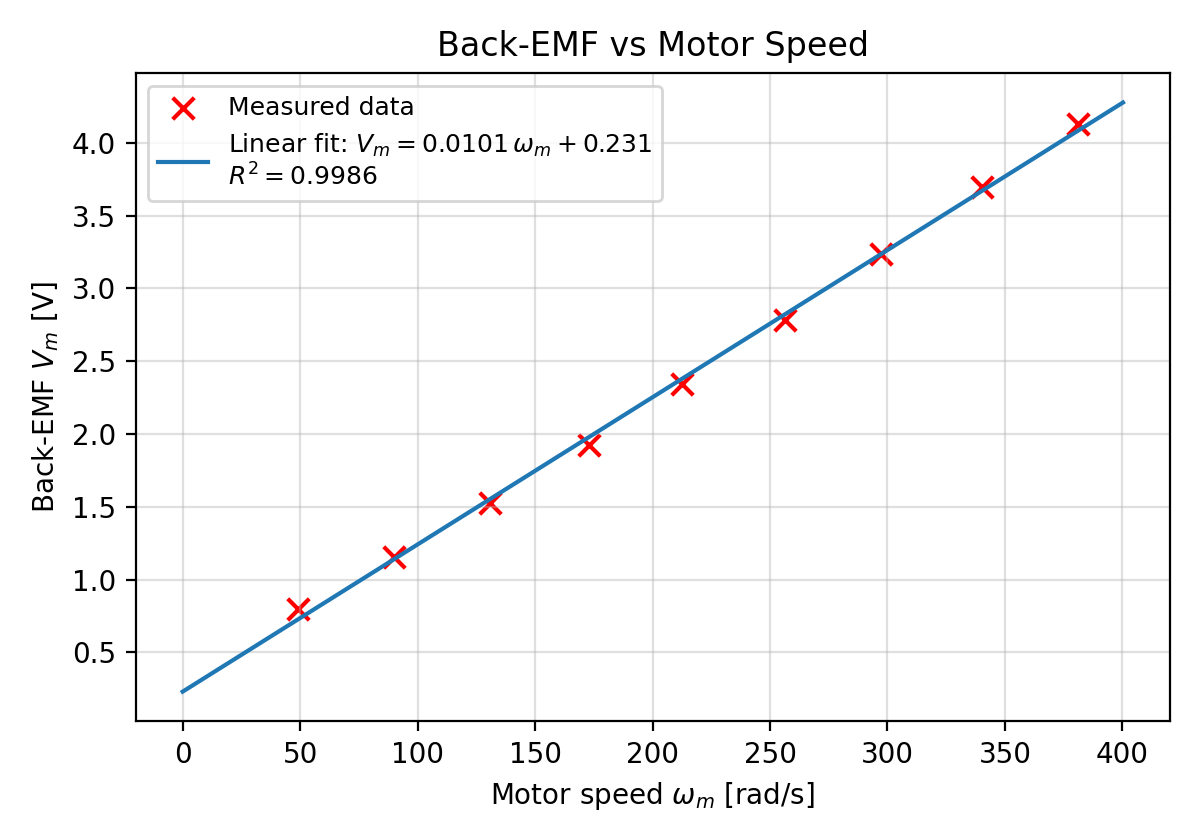
\includegraphics[width=0.75\linewidth]{figures/vm_vs_wm.png}
    \caption{Back-EMF $V_m$ vs.\ motor speed $\omega_m$. The slope of the linear fit is the motor constant $r_m$.}
    \label{fig:vm_vs_wm}
\end{figure}

% =======================================================
\section{Rotational Damping and Friction Torque}
% =======================================================

Without external load, the only torque opposing the electromagnetic torque is the motor's internal friction. Modelling the internal friction as a linear viscous term plus a constant Coulomb term, the effort balance on the motor shaft can be represented as:
\begin{align}
    \tau_{\text{f}}(\omega_m)
    \;=\; B_m\, \omega_m \;+\; \tau_c \\
    \tau_m \;=\; r_m\, i_m
    \;=\; B_m\, \omega_m \;+\; \tau_c
\end{align}

\noindent Under no-load conditions the electromagnetic torque is consumed entirely by viscous damping and by the Coulomb friction torque. Plotting $\tau_m$ against $\omega_m$ at several speeds and performing a linear regression therefore produces a line whose slope is the viscous damping coefficient $B_m$ and intercept is the Coulomb friction torque $\tau_c$. Using the measured multimeter currents at the operating PWMs, computing $\tau_m$ at each point and performing the linear regression in \texttt{Motor\_Characterization\_Student.py}:
\begin{equation}
    \boxed{\;
    B_m \;=\; 4.71\times 10^{-7}~\mathrm{N\!\cdot\!m\!\cdot\!s/rad}
    \qquad
    \tau_c \;=\; 9.81\times 10^{-5}~\mathrm{N\!\cdot\!m}
    \;}
    \label{eq:bm_values}
\end{equation}
with $R^2 = 0.89$. Both values are in SI units: $B_m$ in $\mathrm{N\!\cdot\!m\!\cdot\!s/rad}$ and $\tau_c$ in $\mathrm{N\!\cdot\!m}$. Physically, the small magnitude of $B_m$ relative to $\tau_c$ is the expected behavior, and most of the no-load loss appears as a roughly speed-independent Coulomb friction torque, while the viscous component contributes only a few percent of $\tau_m$ over the tested speed range.

\begin{figure}[H]
    \centering
    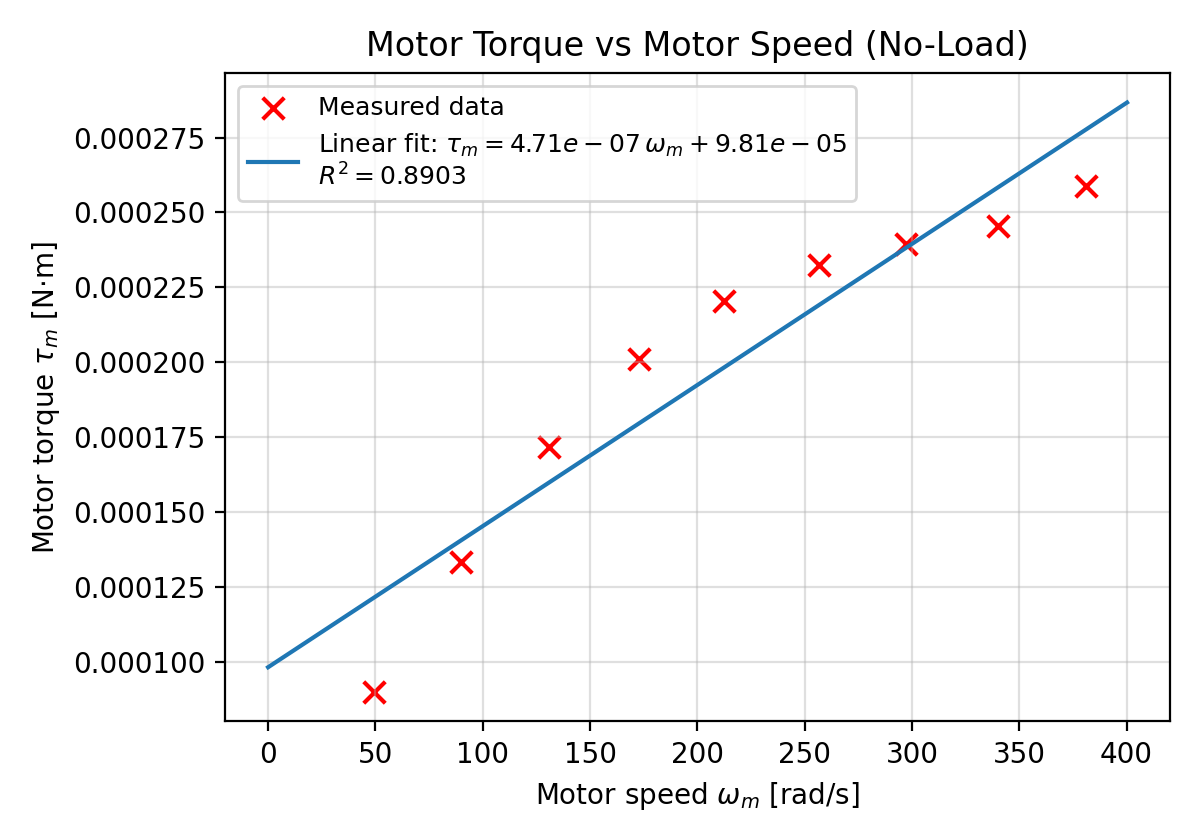
\includegraphics[width=0.75\linewidth]{figures/tm_vs_wm.png}
    \caption{Motor torque $\tau_m = r_m\, i_m$ vs.\ motor speed $\omega_m$. Slope of linear fit gives the viscous damping $B_m$, and the $y$-intercept gives $\tau_c$.}
    \label{fig:tm_vs_wm}
\end{figure}

% =======================================================
\section{Modeled Output Torque-Speed Curves}
% =======================================================

The steady-state torque at the gearbox output is determined by combining equations 1, 3 and the gear reduction $\omega_o = \omega_m / GR$, $\tau_o = GR\,\tau_m$. After substituting and grouping the speed-dependent terms together, the result becomes:

\begin{equation}
    \boxed{\;
    \tau_o(\omega_o)
    \;=\; GR\!\left[\,\frac{r_m}{R_m}\,V_{in}
                  \;-\; GR\!\left(\frac{r_m^{\,2}}{R_m} + B_m\right)\omega_o\,\right]
    \;}
    \label{eq:torque_speed_user}
\end{equation}

\noindent Expanding the bracket gives the form:
\begin{equation}
    \tau_o(\omega_o)
    \;=\; GR\,\frac{r_m}{R_m}\,V_{in}
    \;-\; GR^{2}\!\left(\frac{r_m^{\,2}}{R_m} + B_m\right)
    \;\omega_o
    \label{eq:torque_speed_expanded}
\end{equation}

\noindent Substituting the measured and extracted parameters, $r_m = 1.011\times 10^{-2}~\mathrm{V\!\cdot\!s/rad}$, $R_m = 26.9~\Omega$, $B_m = 4.71\times 10^{-7}~\mathrm{N\!\cdot\!m\!\cdot\!s/rad}$, $GR = 45$ into equation 9 yields the family of curves in Figure 3. The stall torque and no-load output speed for each operating voltage are listed in Table 1.

\begin{figure}[H]
    \centering
    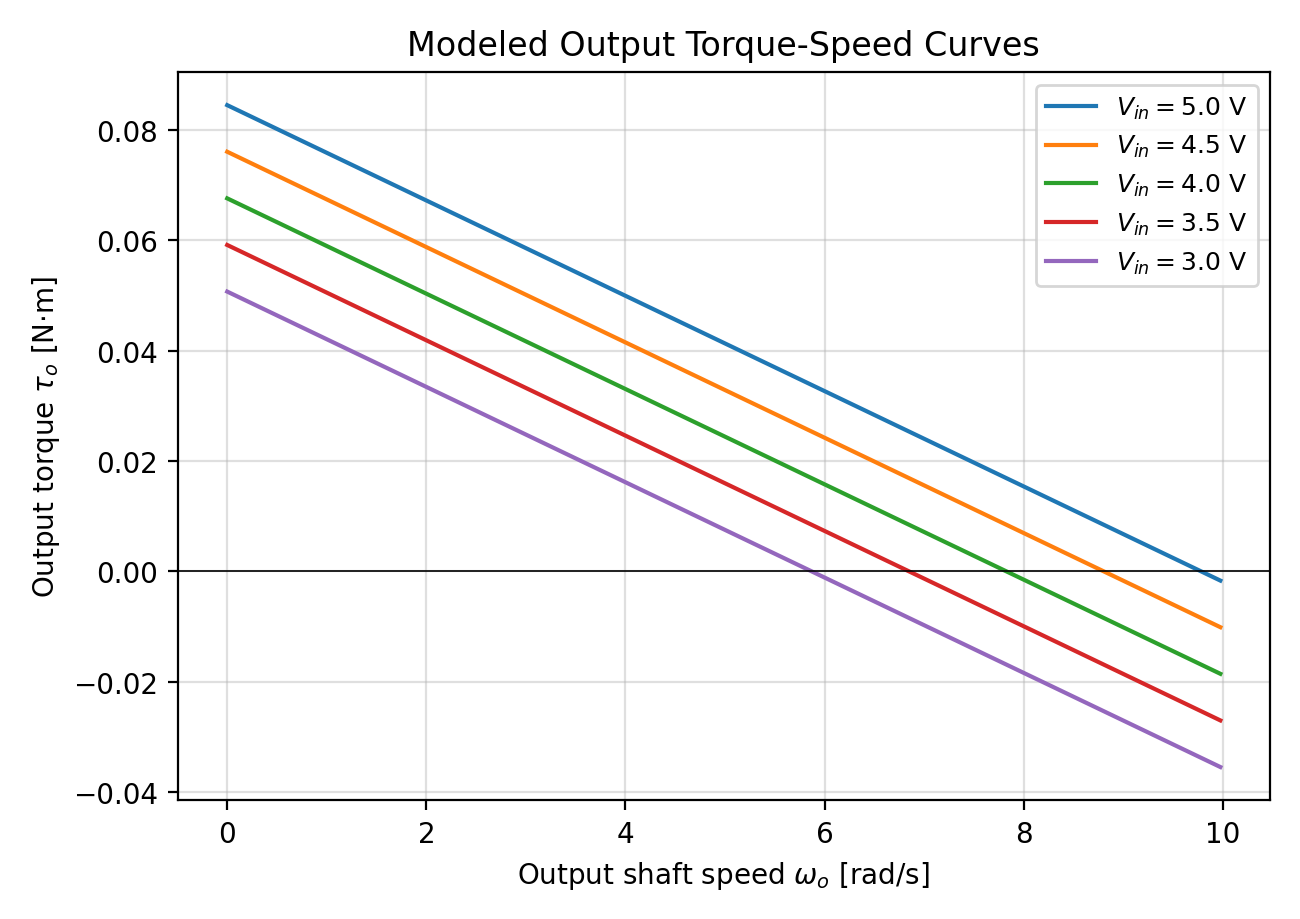
\includegraphics[width=0.85\linewidth]{figures/torque_speed_family.png}
    \caption{Modeled output torque-speed curves $\tau_o$ vs.\ $\omega_o$ for values of $V_{in}$. The curves are parallel, and the stall torque increases linearly with $V_{in}$.}
    \label{fig:torque_speed_family}
\end{figure}

\begin{table}[H]
    \centering
    \caption{Stall torque and no-load output speed predicted by equation 9 at each operating voltage.}
    \label{tab:tscurves}
    \begin{tabular}{cccc}
        \toprule
        $V_{in}$~[V] & $\tau_{o,\text{stall}}$~[N$\cdot$m] & $\omega_{o,\text{no-load}}$~[rad/s] & $\omega_{o,\text{no-load}}$~[RPM] \\
        \midrule
        5.0 & $8.45\cdot 10^{-2}$ & 9.78 & 93.4 \\
        4.5 & $7.61\cdot 10^{-2}$ & 8.80 & 84.1 \\
        4.0 & $6.76\cdot 10^{-2}$ & 7.82 & 74.7 \\
        3.5 & $5.92\cdot 10^{-2}$ & 6.85 & 65.4 \\
        3.0 & $5.07\cdot 10^{-2}$ & 5.87 & 56.0 \\
        \bottomrule
    \end{tabular}
\end{table}

\noindent The maximum-voltage curve at $V_{in} = 5~\mathrm{V}$ predicts a no-load output speed of 93.4~RPM, agreeing with the measured value of 80.89~RPM at $V_{in} = 4.82~\mathrm{V}$.

\end{document}